% !TeX spellcheck = de_CH_frami
\section{Spannungsreferenzen (Kap. 15)}
In vielen Anwendungen benötigt man eine Spannung, die unabhängig von Betriebsspannungsschwankungen oder Temperaturänderungen ist.
Eine solche Spannungsquelle wird als Spannungsreferenz bezeichnet.\\
\begin{minipage}[t]{0.2\textwidth}
	\textbf{Spannungsteiler}\\
	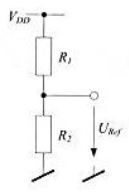
\includegraphics[height=4cm]{chapters/Spannungsref/images/Spannungsteiler}
\end{minipage}
\begin{minipage}[t]{0.2\textwidth}
	\textbf{MOS-Diode}\\
	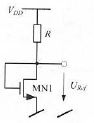
\includegraphics[height=4cm]{chapters/Spannungsref/images/MOS-Diode}
\end{minipage}
\begin{minipage}[t]{0.5\textwidth}
	\textbf{Bandgap-Spannungsreferenz}\\
	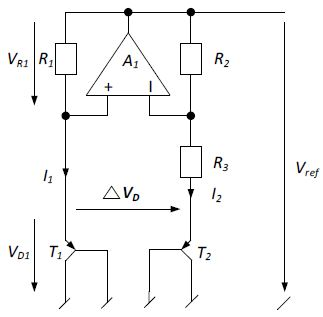
\includegraphics[height=4cm]{chapters/Spannungsref/images/BandgapRealisation}
\end{minipage}\\
\begin{tabular}{|p{2.4cm}|p{4cm}|l|l|}
	\hline
	&\textbf{Temperatur:}&\textbf{VDD/VSS:}&\textbf{Prozessvariation:}\\ \hline
	Spannungsteiler&S klein&$S = 1$&S klein\\ \hline
	MOS-Diode&S klein&$S < 1$&S: Darf nicht vernachlässigt werden.\\ \hline
	Bandgap&Abhängig von $\Phi_t=\frac{kT}{e}$ und von $R$&0 (unabhängig von VDD/VSS)&Klein\\ \hline
\end{tabular}\\
\subsection{Bandgap-Spannungsreferenz}
In vielen Anwendungen benötigt man eine Spannung, die unabhängig von Betriebsspannungsschwankungen oder Temperaturänderungen ist.
Die Bandgap ist eine Möglichkeit, eine stabile Spannungsreferenz zu erhalten.\\
\begin{minipage}[c]{0.5\textwidth}
	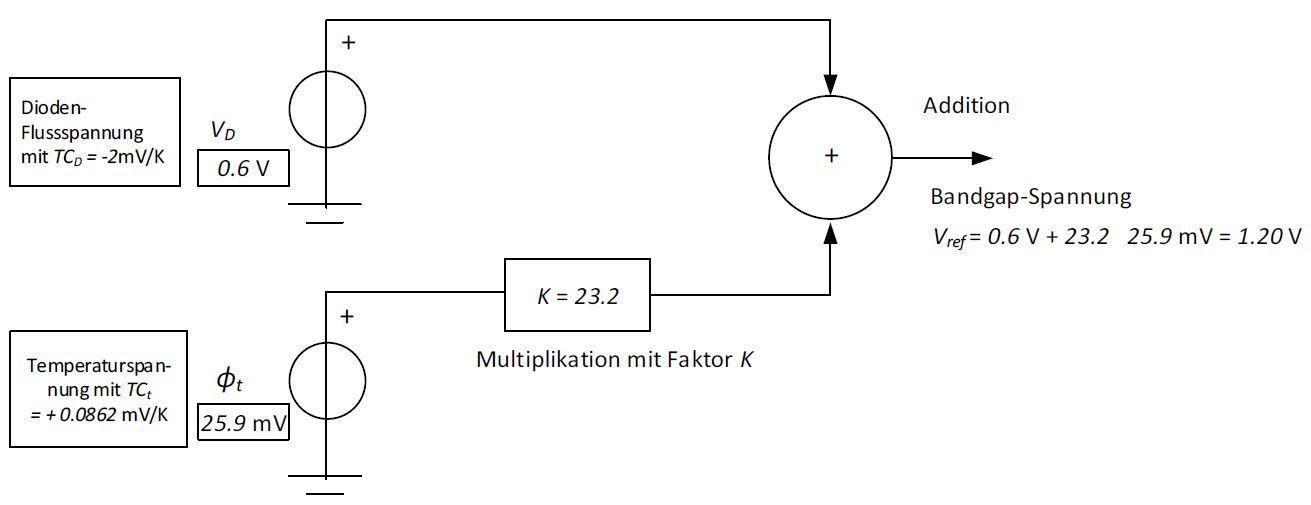
\includegraphics[width=1\linewidth]{chapters/Spannungsref/images/Bandgap}
\end{minipage}
\begin{minipage}[c]{0.5\textwidth}
	\textbf{Formeln:}\\
	$V_{ref} = V_D + K\cdot \Phi_t$\\
	$\Phi_t = \frac{kT}{e}$\\[2ex]
	\textbf{Konstanten:}\\
	$k = \SI{1.38e-23}{\joule / \kelvin}$\\
	T = Absolute Temperatur in K\\
	$e = \SI{1.60e-19}{\coulomb}$\\
	Bei Raumtemperatur ($T=\SI{300}{\kelvin}$ bzw. $\SI{27}{\degreeCelsius}$) ist $\Phi_t = \SI{25.9}{\milli\volt}$
\end{minipage}
\subsubsection{Realisierung}
\begin{minipage}[c]{0.5\textwidth}
	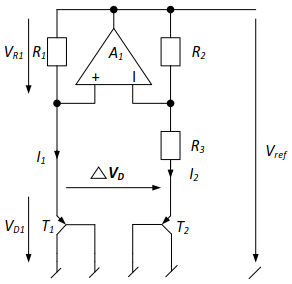
\includegraphics[width=1\linewidth]{chapters/Spannungsref/images/realisierung}
\end{minipage}
\begin{minipage}[c]{0.5\textwidth}
	\textbf{Formeln:}\\
	
\end{minipage}